% Made up for the tikra benchmark.
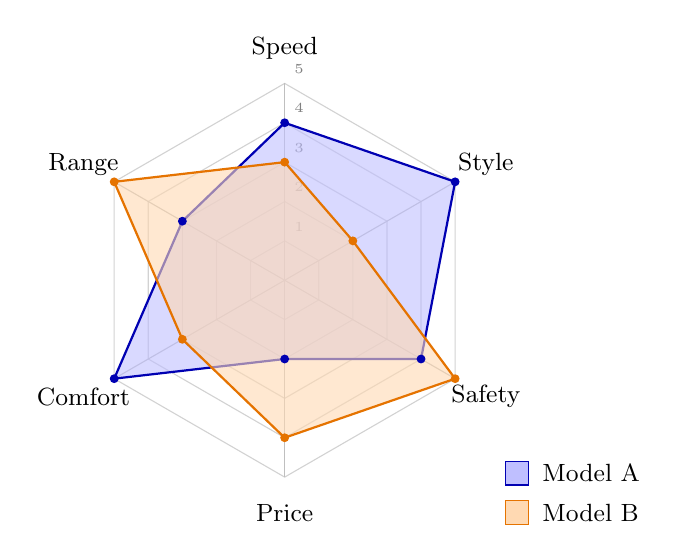
\begin{tikzpicture}[font=\small]
  \def\n{6}
  % web
  \foreach \r in {1,...,5} {
    \draw[gray!35] (90:\r*0.5) \foreach \i in {1,...,5} { -- (90+\i*60:\r*0.5) } -- cycle;
  }
  \foreach \i/\name in {0/Speed, 1/Range, 2/Comfort, 3/Price, 4/Safety, 5/Style} {
    \draw[gray!50] (0,0) -- (90+\i*60:2.5);
    \node at (90+\i*60:2.95) {\name};
  }
  \foreach \r in {1,...,5} { \node[gray, font=\tiny, anchor=south west] at (90:\r*0.5) {\r}; }
  % two products
  \filldraw[blue!70!black, fill=blue!25, fill opacity=0.6, thick]
    (90:2.0) -- (150:1.5) -- (210:2.5) -- (270:1.0) -- (330:2.0) -- (30:2.5) -- cycle;
  \filldraw[orange!90!black, fill=orange!30, fill opacity=0.6, thick]
    (90:1.5) -- (150:2.5) -- (210:1.5) -- (270:2.0) -- (330:2.5) -- (30:1.0) -- cycle;
  \foreach \a/\r in {90/2.0, 150/1.5, 210/2.5, 270/1.0, 330/2.0, 30/2.5} { \fill[blue!70!black] (\a:\r) circle (1.6pt); }
  \foreach \a/\r in {90/1.5, 150/2.5, 210/1.5, 270/2.0, 330/2.5, 30/1.0} { \fill[orange!90!black] (\a:\r) circle (1.6pt); }
  \fill[blue!25, draw=blue!70!black] (2.8,-2.6) rectangle ++(0.3,0.3) node[right, black, pos=0.5, xshift=4pt] {};
  \node[anchor=west] at (3.15,-2.45) {Model A};
  \fill[orange!30, draw=orange!90!black] (2.8,-3.1) rectangle ++(0.3,0.3);
  \node[anchor=west] at (3.15,-2.95) {Model B};
\end{tikzpicture}
